\documentclass[11pt,a4paper]{article}
\newcommand{\Rodzaj}{Szablon sprawozdania — A}
\usepackage{fontspec}
\setmainfont{texgyretermes-regular.otf}[BoldFont=texgyretermes-bold.otf,ItalicFont=texgyretermes-italic.otf]
\usepackage[polish]{babel}
\usepackage{amsmath,amssymb,geometry,array,tabularx,graphicx,caption,fancyhdr}
\usepackage[table]{xcolor}
\geometry{left=18mm,right=18mm,top=19mm,bottom=19mm,headheight=14pt,headsep=6mm}
\setlength{\parindent}{0pt}\setlength{\parskip}{5pt}
\setlength{\emergencystretch}{2em}
\renewcommand{\arraystretch}{1.3}\setlength{\tabcolsep}{5pt}
\setlength{\fboxsep}{6pt}
\setlength{\abovedisplayskip}{8pt}\setlength{\belowdisplayskip}{8pt}
\setlength{\abovedisplayshortskip}{5pt}\setlength{\belowdisplayshortskip}{5pt}
\widowpenalty=10000\clubpenalty=10000
\raggedbottom
\newcolumntype{Y}{>{\raggedright\arraybackslash}X}
\newcolumntype{C}{>{\centering\arraybackslash}X}
\newcommand{\naglowek}{\rowcolor{gray!12}}
\newcommand{\odstep}{\par\smallskip}
\captionsetup{font=small,labelfont=bf,justification=justified,singlelinecheck=false}
\pagestyle{fancy}\fancyhf{}\fancyhead[L]{\small Ćwiczenie 31 — modelowanie pola}
\fancyhead[R]{\small\Rodzaj}\fancyfoot[C]{\small\thepage}
\renewcommand{\headrulewidth}{0.3pt}
\makeatletter
\renewcommand\section{\@startsection{section}{1}{0pt}{10pt}{4pt}{\large\bfseries}}
\renewcommand\subsection{\@startsection{subsection}{2}{0pt}{8pt}{4pt}{\normalsize\bfseries}}
\makeatother
\newcommand{\pole}{\rule{23mm}{0.3pt}}
\newcommand{\miejsce}[2]{\par\medskip\noindent\fbox{\begin{minipage}[t][#1][t]{\dimexpr\linewidth-2\fboxsep-2\fboxrule\relax}\small #2\end{minipage}}\par\medskip}
\newcommand{\metryka}{%
\begingroup\small\setlength{\parskip}{0pt}\renewcommand{\arraystretch}{1.1}
\begin{tabularx}{\linewidth}{|p{29mm}|Y|p{18mm}|p{18mm}|p{19mm}|}\hline
\textbf{Wydział}\newline Informatyki & \textbf{Imię i nazwisko}\newline 1. Marcin Podyma\newline 2. Paweł Mierzwa & \textbf{Rok}\newline 2026 & \textbf{Grupa}\newline 3 & \textbf{Zespół}\newline 1\\\hline
\end{tabularx}\par\nointerlineskip
\begin{tabularx}{\linewidth}{|p{29mm}|Y|p{19mm}|}
\parbox[t]{29mm}{\centering\textbf{PRACOWNIA\\FIZYCZNA\\WFiIS AGH}} & \textbf{Temat:}\newline Modelowanie pola elektrycznego & \textbf{Nr}\newline\textbf{ćwiczenia}\newline 31\\\hline
\end{tabularx}\par\nointerlineskip
\begin{tabularx}{\linewidth}{|p{29mm}|Y|Y|Y|Y|p{19mm}|}
\textbf{Data wykonania}\newline\strut & \textbf{Data oddania}\newline\strut & \textbf{Zwrot do popr.} & \textbf{Data oddania} & \textbf{Data zaliczenia} & \textbf{OCENA}\\\hline
\end{tabularx}\endgroup\medskip}



\newcommand{\podstawy}{%
\par\smallskip
Na jednorodnym papierze przewodzącym stacjonarny przepływ prądu
modeluje pole elektrostatyczne w obszarze bez ładunków, jeśli odpowiadają
sobie warunki brzegowe. Potencjał spełnia równanie Laplace'a.
\[
\boxed{\nabla^2V=0,\qquad \mathbf E=-\nabla V,\qquad
|\mathbf E|=\sqrt{E_x^2+E_y^2}.}
\]
Linie pola są prostopadłe do ekwipotencjalnych i skierowane od wyższego
potencjału do niższego. Wartość natężenia i składowa ze znakiem to różne wielkości.
}
\newcommand{\teoriaA}{%
\par\smallskip
Dla idealnych równoległych elektrod przy $V(0)=0$ i $V(d)=U$:
\[
\boxed{V(x)=\frac Ud x,\qquad E_x=-\frac Ud,\qquad |\mathbf E|=\frac Ud.}
\]
Zależność opisuje wnętrze z pominięciem efektów brzegowych;
poza elektrodami pole jest niejednorodne.
}
\newcommand{\teoriaB}{%
\par\smallskip
Dla elektrody wewnętrznej o promieniu $r_w$ i potencjale $U$
oraz zewnętrznej $r_z$ o potencjale 0:
\[
\boxed{V(r)=U\frac{\ln(r_z/r)}{\ln(r_z/r_w)},\qquad
E_r(r)=\frac{U}{r\ln(r_z/r_w)}.}
\]
Wtedy $V(r_w)=U$, $V(r_z)=0$, a pole jest skierowane na zewnątrz.
Odwrócenie biegunowości odwraca wektor. Zmiana zera potencjału
o stałą nie zmienia pola; nie jest tym samym co zmiana znaku całego $V$.
}
\newcommand{\teoriaC}{%
\par\smallskip
Dla dowolnego układu elektrod nie zakładamy postaci liniowej ani
radialnej. Linie wyznaczamy z pomiarów potencjału i warunków na elektrodach.
Obszary bez danych oznaczamy, nie wypełniając ich fikcyjnymi pomiarami.
}
\newcommand{\roznice}{%
\par\smallskip
Dla trzech kierunków w tej samej odległości:
\[
\boxed{\bar V_i=\frac{V_{a,i}+V_{b,i}+V_{c,i}}3,\quad
s_i^*=\frac{s_i+s_{i+1}}2,\quad
E_{s,i}=-\frac{\bar V_{i+1}-\bar V_i}{s_{i+1}-s_i}.}
\]
Współrzędna $s$ oznacza $x$ lub $r$. W mianowniku używaj metrów:
$1\ \mathrm{mm}=10^{-3}\ \mathrm m$. Przypisz pochodną do środka przedziału.
Trzy kierunki nie muszą być trzema niezależnymi powtórzeniami tego samego pomiaru.
}
\newcommand{\mapowanie}{%
Linie ekwipotencjalne rysuj co 1--2 V. Szukane położenie między
zmierzonymi punktami wyznacz przez interpolację, nie przez zastąpienie
pomiarów idealnym polem. Dla sąsiadów odległych o $h,k$:
\[
\boxed{E_x\approx-\frac{V(x+h,y)-V(x,y)}h,\qquad
E_y\approx-\frac{V(x,y+k)-V(x,y)}k.}
\]
Powyższe składowe są różnicami w przód przy punkcie bazowym;
podaj użyte punkty i kroki. Dla wektora w środku komórki użyj
uśrednionych różnic na przeciwległych krawędziach. Nie łącz składowych
liczonych w różnych miejscach bez wyjaśnienia.
}
\newcommand{\dokladnosc}{%
Zapisz specyfikację i zakres woltomierza, krok siatki oraz stabilność
zasilania i kontaktu sondy. Dla niezależnych odczytów i odstępu $\Delta s$:
\[
\boxed{u(E_s)\approx\sqrt{
\frac{u^2(V_i)+u^2(V_{i+1})}{(\Delta s)^2}
+\frac{(V_{i+1}-V_i)^2}{(\Delta s)^4}u^2(\Delta s)}.}
\]
Uwzględnij korelacje, jeśli odczyty mają wspólne odniesienie lub błąd skali.
Bez danych przyrządów nie wpisuj wymyślonych słupków niepewności.
Różniczkowanie nasila wpływ szumu; interpolacja nie zwiększa liczby pomiarów.
}
\newcommand{\parametry}[1]{%
\begin{tabularx}{\linewidth}{|>{\raggedright\arraybackslash}p{55mm}|Y|}\hline
\naglowek\textbf{Parametr wariantu #1} & \textbf{Wpis ze stanowiska}\\\hline
Wariant i oznaczenie płyty &\rule{0pt}{9mm}\\\hline
Napięcia obu elektrod / odniesienie &\rule{0pt}{9mm}\\\hline
Geometria: $d$ albo $r_w,r_z$ &\rule{0pt}{9mm}\\\hline
Krok otworów $h,k$, początek i zwrot osi &\rule{0pt}{9mm}\\\hline
Kierunki a,b,c / kąty promieni &\rule{0pt}{9mm}\\\hline
Woltomierz: model, zakres, dokładność &\rule{0pt}{9mm}\\\hline
\end{tabularx}\par\medskip
Napięcie zalecane w instrukcji: 10 V. Zapisz rzeczywistą wartość
i biegunowość; nie przenoś wymiarów z cudzego przykładu.
}
\newcommand{\aparatura}{%
\par\medskip\noindent
\begin{minipage}[c]{.49\linewidth}\centering
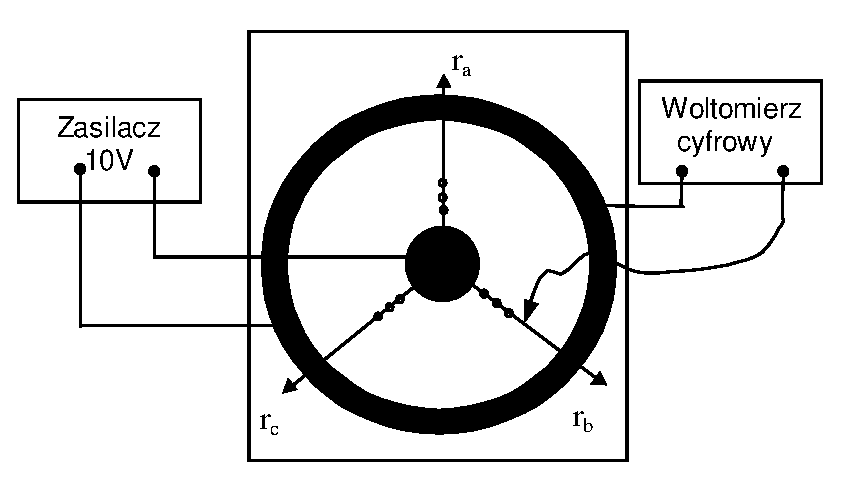
\includegraphics[width=\linewidth]{../../Wspolne/Rysunki/uklad.pdf}
\end{minipage}\hfill
\begin{minipage}[c]{.47\linewidth}
\raggedright
\captionof{figure}{Układ pomiarowy z instrukcji 31\_wykon.pdf, s.~2.}
\smallskip Zasilacz wymusza różnicę potencjałów elektrod.
Woltomierz z sondą mierzy napięcie wybranego punktu względem
ustalonej elektrody odniesienia. Papier przewodzący stanowi model pola.
Wymiana płyty zmienia geometrię elektrod, nie zasadę pomiaru.
\end{minipage}\par\medskip}

\begin{document}\metryka
\section{Cel ćwiczenia}
Wyznaczenie potencjału, linii ekwipotencjalnych i wektorów pola dla układu: kondensator płaski.
\section{Podstawy teoretyczne}\podstawy
\teoriaA
\clearpage\section{Aparatura i przebieg}\aparatura\parametry{A}
\miejsce{30mm}{Opisz rzeczywiste połączenia, pomiar odniesienia, geometrię i wybór punktów; nie kopiuj przebiegu cudzej serii.}
\clearpage\section{Wyniki pomiarów}
\par\medskip\begingroup\small\noindent\begin{tabularx}{\linewidth}{|c|Y|Y|Y|Y|}\hline
\naglowek Nr & $x$ lub $r$ [mm] & $V_a$ [V] & $V_b$ [V] & $V_c$ [V]\\\hline
1 &  &  &  & \rule{0pt}{7mm}\\\hline
2 &  &  &  & \rule{0pt}{7mm}\\\hline
3 &  &  &  & \rule{0pt}{7mm}\\\hline
4 &  &  &  & \rule{0pt}{7mm}\\\hline
5 &  &  &  & \rule{0pt}{7mm}\\\hline
6 &  &  &  & \rule{0pt}{7mm}\\\hline
7 &  &  &  & \rule{0pt}{7mm}\\\hline
8 &  &  &  & \rule{0pt}{7mm}\\\hline
9 &  &  &  & \rule{0pt}{7mm}\\\hline
10 &  &  &  & \rule{0pt}{7mm}\\\hline
11 &  &  &  & \rule{0pt}{7mm}\\\hline
12 &  &  &  & \rule{0pt}{7mm}\\\hline
13 &  &  &  & \rule{0pt}{7mm}\\\hline
14 &  &  &  & \rule{0pt}{7mm}\\\hline
15 &  &  &  & \rule{0pt}{7mm}\\\hline\end{tabularx}\endgroup\par\medskip
\miejsce{25mm}{Średnie potencjały i wartości teoretyczne dla każdej współrzędnej. Przy większej liczbie pomiarów rozszerz tabelę.}
\clearpage\section{Potencjał i natężenie}\roznice
\par\medskip\begingroup\small\noindent\begin{tabularx}{\linewidth}{|c|Y|Y|Y|}\hline
\naglowek Nr & $x^*$ lub $r^*$ [mm] & $E_{s,\mathrm{dosw}}$ [V/m] & $E_{s,\mathrm{teor}}$ [V/m]\\\hline
1 &  &  & \rule{0pt}{7mm}\\\hline
2 &  &  & \rule{0pt}{7mm}\\\hline
3 &  &  & \rule{0pt}{7mm}\\\hline
4 &  &  & \rule{0pt}{7mm}\\\hline
5 &  &  & \rule{0pt}{7mm}\\\hline
6 &  &  & \rule{0pt}{7mm}\\\hline
7 &  &  & \rule{0pt}{7mm}\\\hline
8 &  &  & \rule{0pt}{7mm}\\\hline\end{tabularx}\endgroup\par\medskip
\miejsce{46mm}{Wykres potencjału: dane trzech kierunków, ich średnia i linia teoretyczna; osie z jednostkami.}
\miejsce{46mm}{Wykres natężenia: punkty w połowach przedziałów, właściwy znak składowej i porównanie z teorią.}
\clearpage\section{Linie ekwipotencjalne i wektory pola}
\mapowanie
\miejsce{95mm}{Mapa: punkty pomiarowe, elektrody i osie, linie ekwipotencjalne co 1–2 V, linie pola z kierunkiem. Rozróżnij interpolację pomiarów od mapy teoretycznej.}
\par\medskip\begingroup\small\noindent\begin{tabularx}{\linewidth}{|c|Y|Y|Y|Y|}\hline
\naglowek Nr & $x,y$ [mm] & $E_x$ [V/m] & $E_y$ [V/m] & $|\mathbf E|$ [V/m]\\\hline
1 &  &  &  & \rule{0pt}{8mm}\\\hline
2 &  &  &  & \rule{0pt}{8mm}\\\hline
3 &  &  &  & \rule{0pt}{8mm}\\\hline
4 &  &  &  & \rule{0pt}{8mm}\\\hline
5 &  &  &  & \rule{0pt}{8mm}\\\hline\end{tabularx}\endgroup\par\medskip
\clearpage\section{Dokładność i dyskusja}\dokladnosc
\miejsce{35mm}{Podaj rozbieżności danych i modelu: wartości, obszary, możliwe przyczyny i ograniczenia. Nie stwierdzaj zgodności tylko na podstawie podobnego kształtu wykresu.}
\section{Wnioski}
\par\medskip\begingroup\small\noindent\begin{tabularx}{\linewidth}{|c|Y|}\hline
\naglowek Nr & Wynik i interpretacja\\\hline
1 & \rule{0pt}{16mm}\\\hline
2 & \rule{0pt}{16mm}\\\hline
3 & \rule{0pt}{16mm}\\\hline
4 & \rule{0pt}{16mm}\\\hline\end{tabularx}\endgroup\par\medskip
\end{document}